\documentclass[11pt]{article}

\usepackage{common}
\usepackage{booktabs}
\usepackage{wrapfig}
\usepackage{titling}
\usepackage{titlesec}
\usepackage{float}
\usepackage[margin=0.99in]{geometry}

\titlespacing\section{0pt}{4pt}{2pt}
\setlength{\parskip}{0.35em}
\setlength{\droptitle}{-5em}
\pagestyle{plain}


\title{Practical 2: Classification\\ Classifying Malicious Software}
\author{Antonio Copete, acopete@cfa.harvard.edu, Camelot.ai Copete \\
	Fangli Geng, fgeng@g.harvard.edu, Camelot.ai fangligeng\\
	Junran Yang, jyang3@gsd.harvard.edu, Camelot.ai junran}

\begin{document}
\maketitle{}

\section{Technical Approach}

The purpose of this practical was to classify a test set of 3,724 files in XML format into 15 classes of malware, using a training set of 3,086 labeled files. Our general approach consisted on the following steps:

\begin{enumerate} %[leftmargin=1cm]

\item \textbf{Feature Engineering}\\
Initial inspection showed the XML data files to be structured hierarchically into a series of \emph{processes}, in turn composed of a series of \emph{threads}, in turn composed of a series of \emph{system calls}. Each of these were identified by a \emph{tag} as well as a number of \emph{attributes} indicated as sets of key-value pairs. Our simplest approach began by drawing $n$-grams (ordered sets) of up to 4 consecutive system call tags, initially without attributes, and our initial exploratory analysis tested the hypothesis that the presence and order of such system call tags was correlated with the distinct anomalous behavior found in different types of malware.

More advanced versions of this approach found in the literature \cite{canali} suggested also drawing features based on $n$-bags (unordered non-consecutive sets) as well as $n$-tuples (ordered non-consecutive sets) of system calls and processes, as well as including attributes such as file names, file sizes, URLs, execution times, etc. We found some of these attributes to be oddly predictive of some specific classes, such as the file \verb|maxtrox.txt| being always related to malware of class VB, and \verb|GrayPigeon_Hacker.com.cn| always indicating malware of class Hupigon. In addition, we also took the number of total processes and thread numbers into account.

To analyze the system call tags (including 4-grams, 29,813 features in total) and predictive attributes (110,465 features in total), we tried 2 methods: using either the number of counts, or the TF-IDF (term frequency---inverse document frequency) \cite{canzanese}. The TF-IDF value measures the relative frequency of a token across the data set; it is proportional to the number of times a token appears in a given file, offset by the frequency of the token across all files, which helps adjust for the absolute frequency of a given token in the whole dataset. The scikit-learn module \verb|sklearn.feature_extraction.text| includes the objects \verb|CountVectorizer| and \verb|TfidfVectorizer|, which tokenize large strings of tags (with or without arguments) into $n$-grams, and then transform them into counts and TF-IDF values in the resulting feature matrix, respectively.


\item \textbf{Feature Selection}\\
Since we derived roughly 140,000 features from a training set of just over 3,000 files, it was easy to cause our model to overfit the data. To avoid overfitting, we used the sklearn module \verb|SelectFromModel| and the classifier \verb|sklearn.ensemble.RandomForestClassifier| to reduce features and use cross-validation to determine the features we wanted to keep. More specifically, we ran a loop to continuously drop features with importance of less than 10\% the mean importance among all features, monitoring the mean score from 5-fold cross-validation in each iteration. The highest score happened with around 5,000 features, which was 1/20 of the original feature size.
% Antonio: I also dropped features with low variance across both the training and test set (unsupervised feature selection), and used a similar strategy to drop features according to RF importance. I went more conservatively and dropped only features that had importance = 0 in all 5 cross-validation sets. But Fangli's strategy is good, so we can leave it at that.

\item\textbf{Model Selection}\\
We began by exploring a number of classifiers for model selection from scikit-learn, including \verb|RandomForestClassifier| (Random Forest), \verb|svm.SVC| and \verb|svm.LinearSVC| (Support Vector), and \verb|linear_model.SGDClassifier| (Stochastic Gradient Descent), with default hyper-parameters. The Random Forest classifier yielded the best score of 0.78105 on the test data, compared to 0.57211 for SVC, 0.76789 for Linear SVC, and 0.77158 for SGD. We thus selected Random Forest as our main model and proceeded to tune it in the subsequent steps.

In addition, we found the class distribution in the training set to be heavily imbalanced. We therefore took a sequential approach to model training, dividing the data into 4 main categories: None (52.14\%), Swizzor (17.56\%), VB (12.18\%) and Others (18.12\%). We first trained the model on each of first 3 categories, and then separately on the minor categories. This approach resulted in an improvement of 0.02 in the test score, compared to training on all categories jointly (0.81211 vs 0.79263). We tried the same approach on a Neural Network for comparison, which yielded a score of 0.79105 for training on separate categories, and confirming again Random Forest as the better model to choose.

Late in the process, we also found a bug in the original code we were provided for extracting system call tags, which was causing the tags for every other thread to be skipped altogether. Our final results are based on the corrected version of feature extraction, but due to time constraints we limited ourselves to 4-gram tokens of system call tags without attributes. With the corrected feature set and a Random Forest classifier trained jointly across all categories, we obtained an improvement of 0.015 in the test data score (0.80789 vs 0.79263).

In our last attempt at model experimentation, we were inspired by a Microsoft Malware Classification Challenge (BIG2015)\footnote{https://www.kaggle.com/c/malware-classification/discussion/13897} to utilize xgboost and a semi-supervised method to detect malware from assembly code. Gradient Boosting is different from Random Forest in that it focuses more on reducing the bias rather than variance. After grid searching for hyperparameters, the highest accuracy we got by xgboost was 0.82526. Furthermore, we tried semi-supervised Gradient Boosting, aiming to further reduce the bias of the model and incorporating information from test dataset into training dataset. We first generate pseudo labels for the test set by selecting the most likely classification based on our best modeling of the training set alone. Then we predict on the test set again in a cross-validation fashion using both the training data and test data.

As an example, consider a test set that is split into 4 folds: A, B, C and D. We draw a new training set that is composed of test folds A, B and C with their pseudo labels, in addition to the original training set, and we then predict on test set fold D. The same method is used to predict on A, B and C. However, this approach didn't provide us with decent results. We suspect the relatively low accuracy in the prediction set (0.82526) provided more inaccurate information than that it could offer to reduce bias.
 
\end{enumerate}

\section{Results}

\begin{table}[htbp]
\centering
\begin{tabular}{cclccccc}
 \toprule
 Rank & \multicolumn{1}{p{1cm}}{\centering Max Depth} & \multicolumn{1}{p{0.8cm}}{\centering $\eta$} & 
 \multicolumn{1}{p{2cm}}{\centering Min. Child Weight} & colsample & \multicolumn{1}{p{2cm}}{\centering CV Mean Error} & 
\multicolumn{1}{p{2cm}}{\centering Best Num. Round} & Final Score\\
 \midrule
  1 & 4 & 0.15 & 1 & 0.5 & 0.093332 & 49 & 0.82158\\
  2 & 6 & 0.2 & 1 & 1 & 0.093334 & 25 & 0.811054\\
  3 & 4 & 0.1 & 1 & 0.5 & 0.093983 & 68 & 0.82526\\
  4 & 4 & 0.15 & 2 & 0.5 & 0.094306 & 54 & - - -\\
  5 & 6 & 0.15 & 1 & 1 & 0.094953 & 31 & - - -\\
 \bottomrule
\end{tabular}
\caption{\label{tab:results} Result tables for the best 5 cross-validation scores by Gradient Boosting with grid search}
\end{table}

Table \ref{tab:results}  shows the best 5 cross-validation scores by Gradient Boosting with grid search. The hyperparameters we tuned were \verb|max_depth| (the maximum depth of a tree, same definition as GBM, set as [2, 4, 6]), $\eta$ (analogous to learning rate in GBM, set as [0.05, 0.1, 0.15, 0.2]),  \verb|min_child_weight| (minimum sum of weights of all observations required in a child, set as [1, 2]), \verb|colsample_bytree| (denotes the subsample ratio of columns for each split, in each level, set as [0.5, 1]). Those 48 possible configurations were drawn from the ones people use most commonly. We also tested models with higher and lower round numbers, optimizing the result by cross-validation.

Figures \ref{fig:results_1}--\ref{fig:results_3} show the results of the tuning process for the Random Forest model for 2 hyperparameters: the maximum tree depth \verb|max_depth|, as well as the number of estimators (trees) \verb|n_estimators|. Results are shown for a validation set (blue) drawn from 20\% of the training data in a stratified fashion (i.e. preserving class proportions), as well as for the remaining training data (red). 

\begin{figure}[H]
\minipage{0.48\textwidth}
  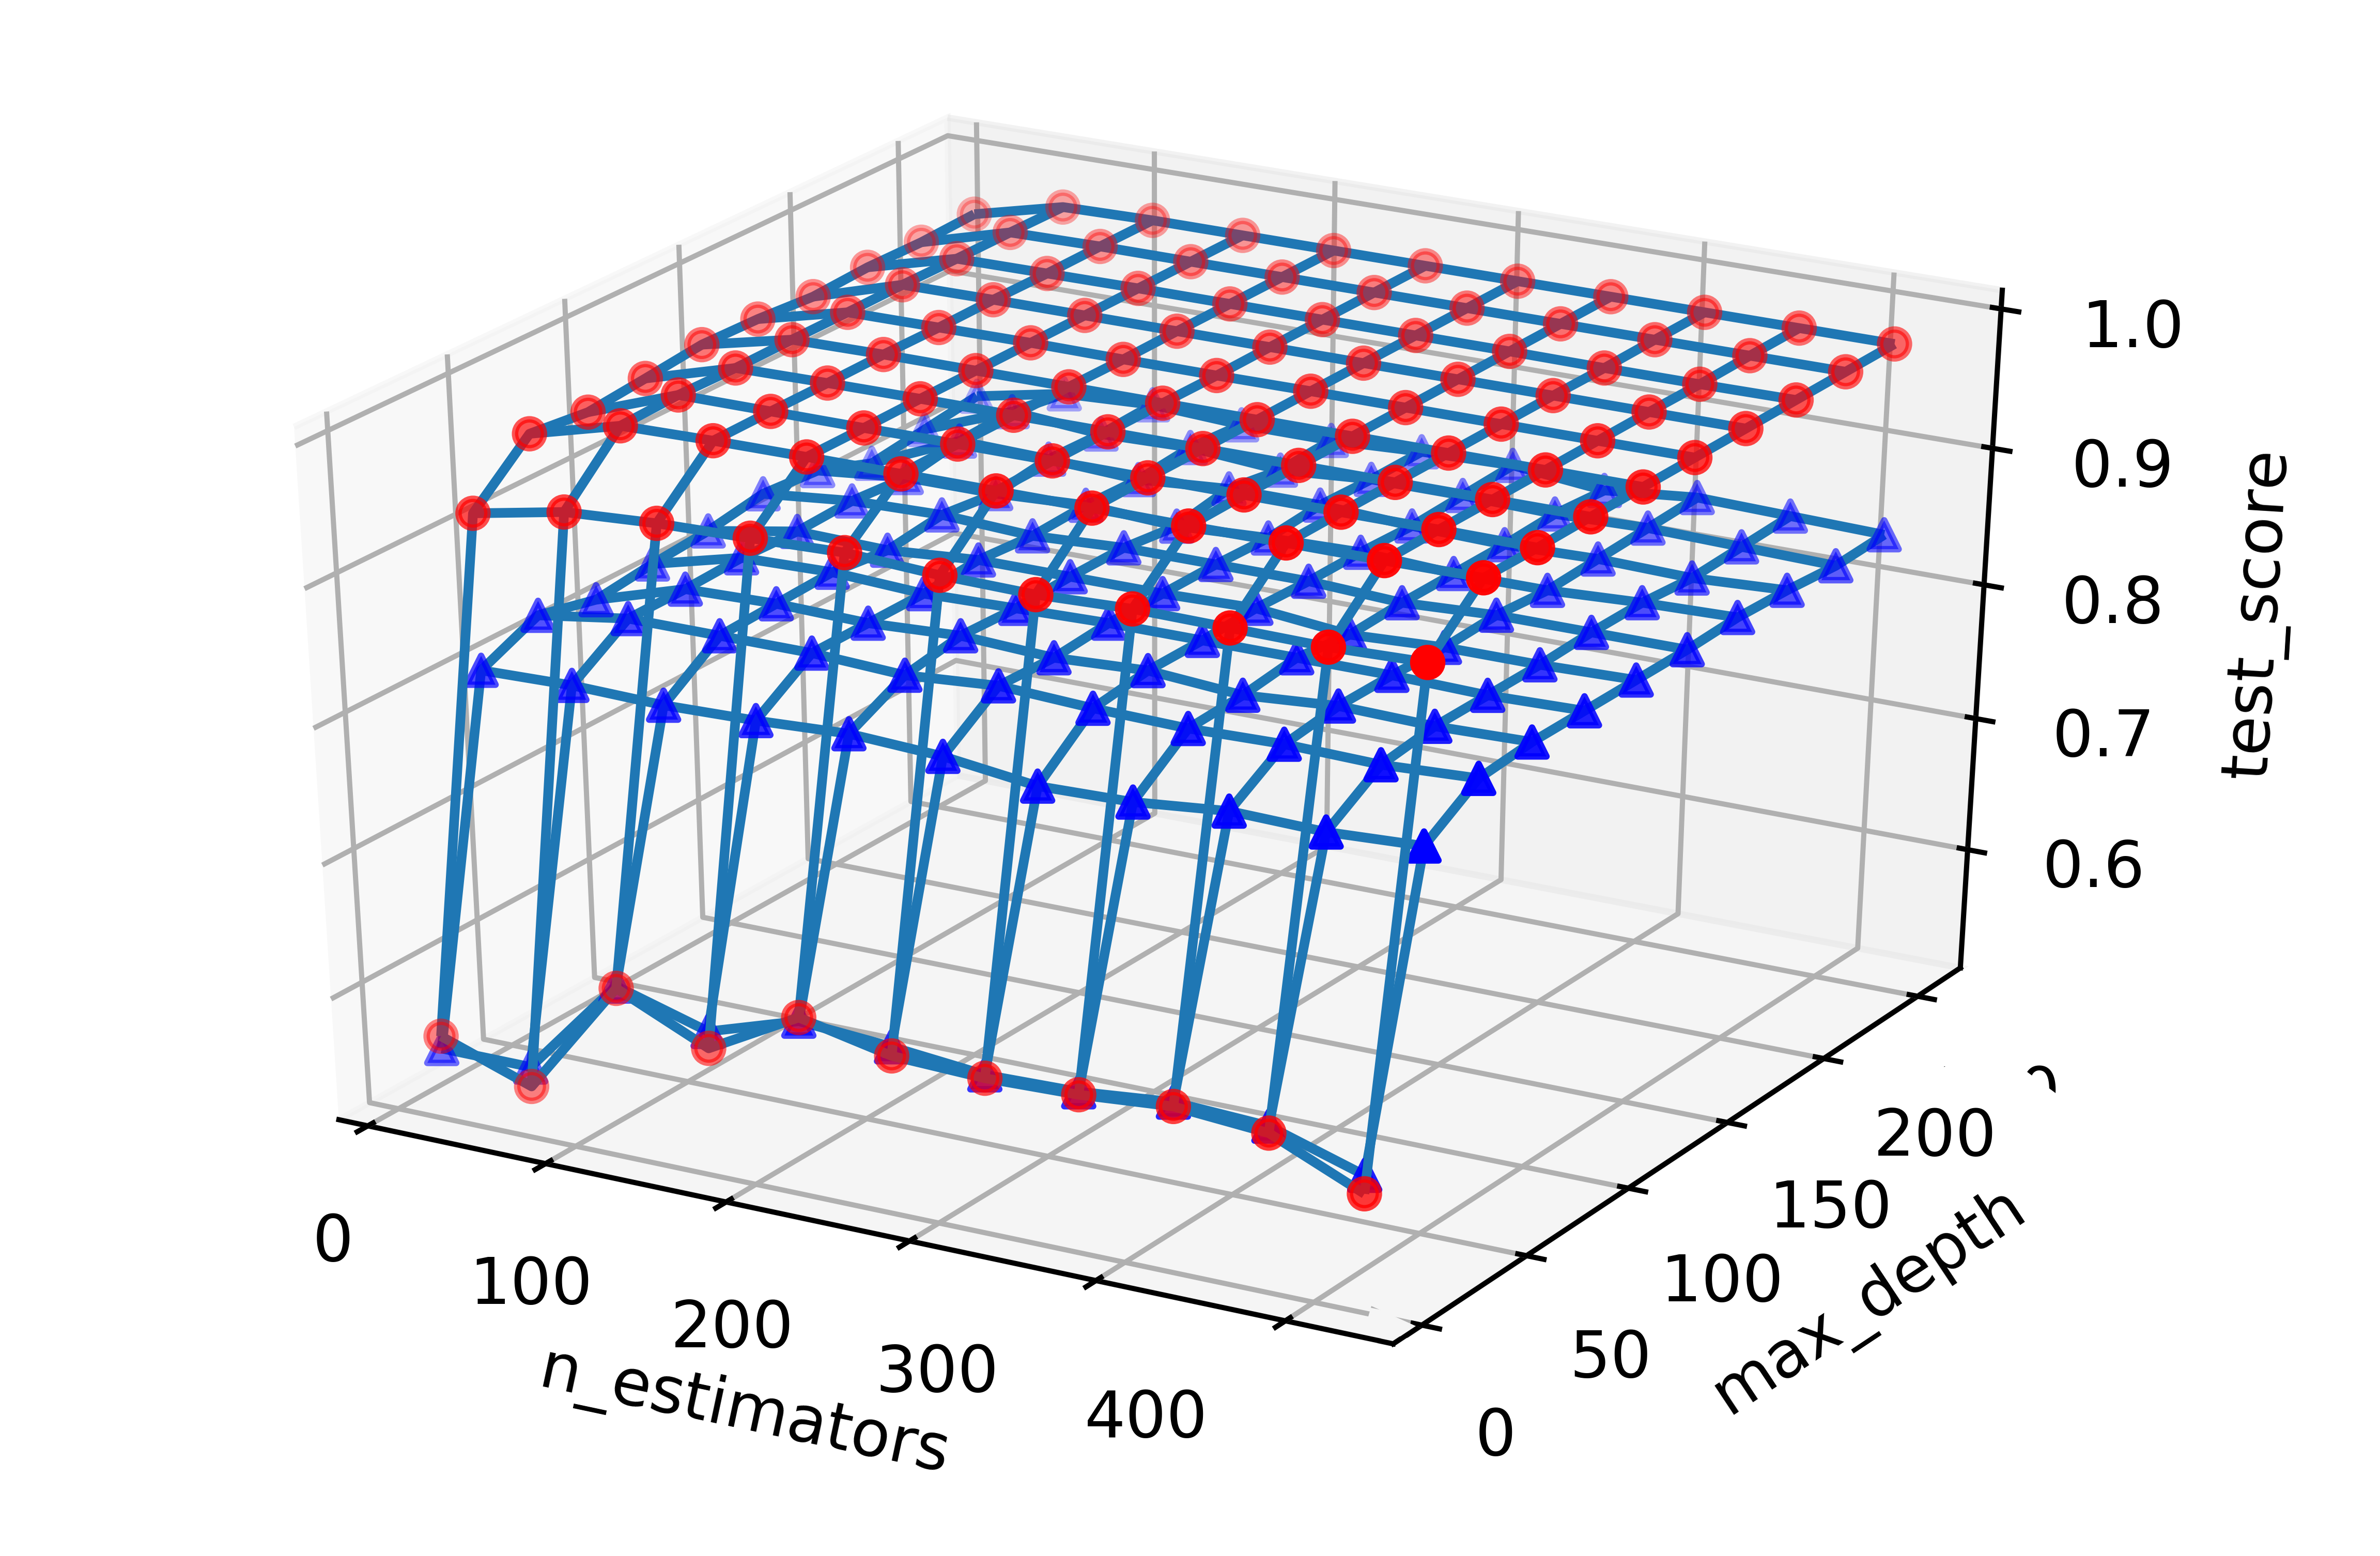
\includegraphics[width=\linewidth]{hyperparameter_tuning_1}
  \caption{Max depth range from 10 to 235, and number of estimators range from 10 to 460.}
  \label{fig:results_1}
\endminipage\hfill
\minipage{0.48\textwidth}
  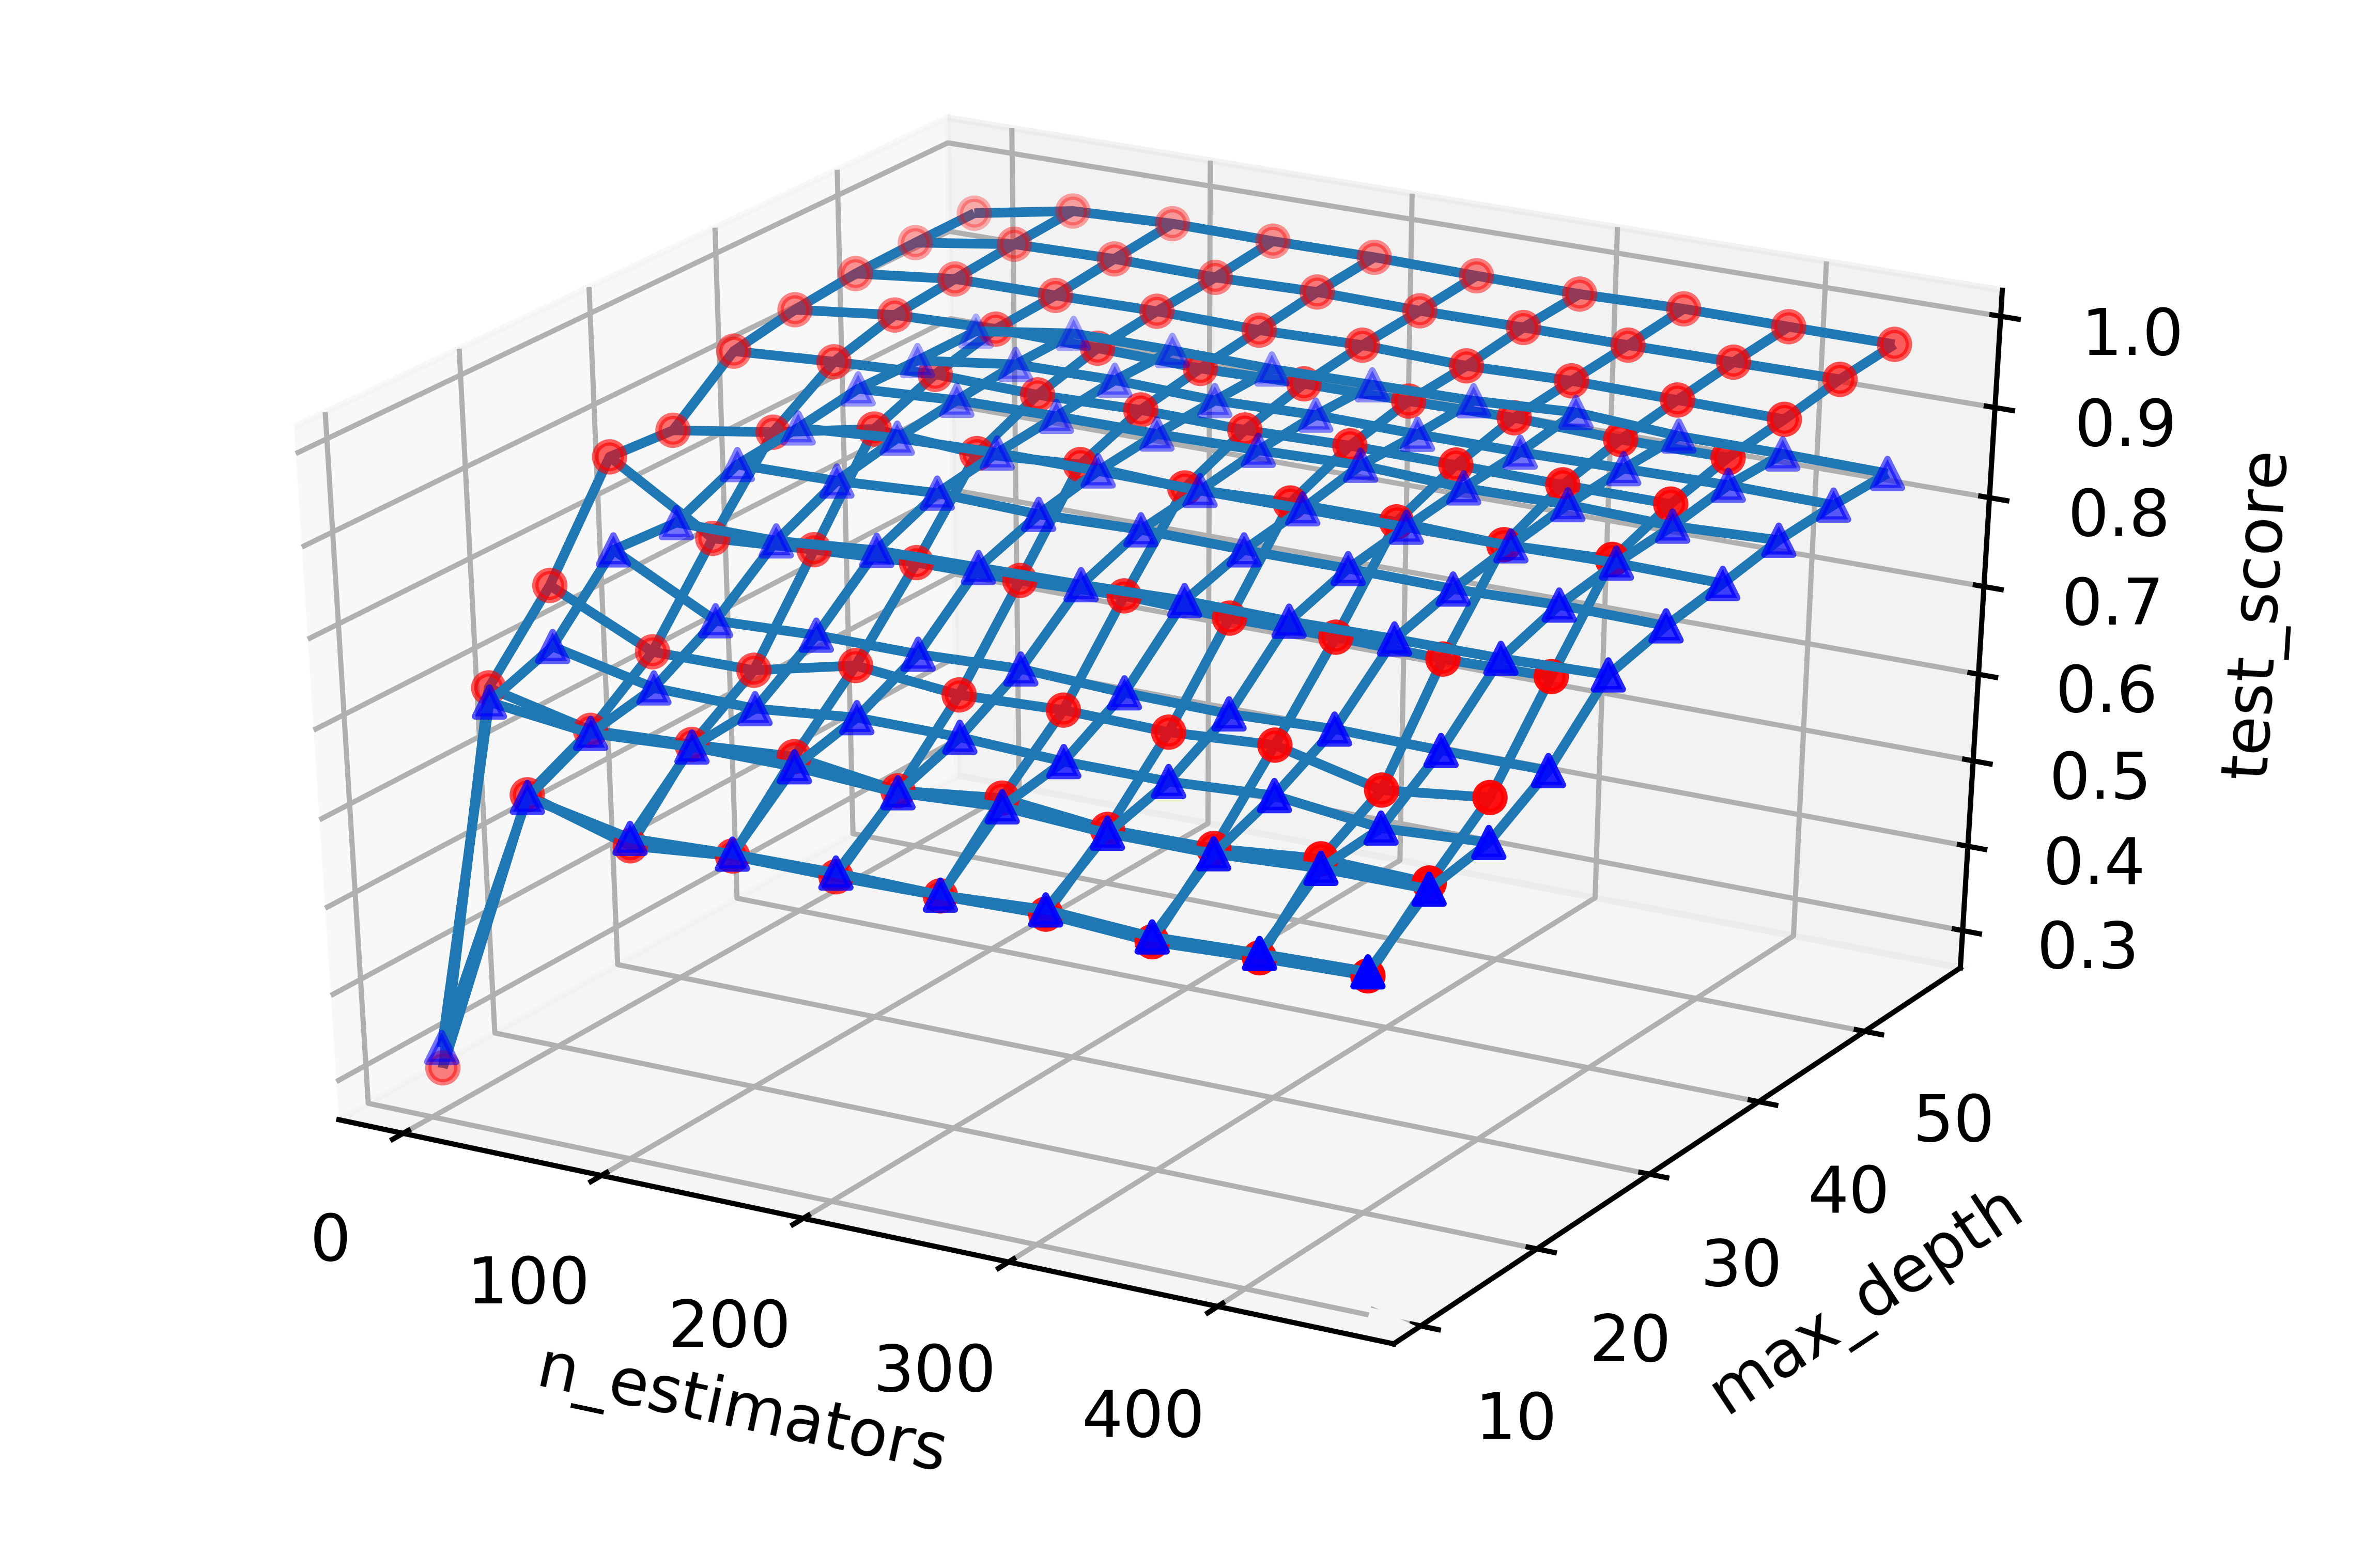
\includegraphics[width=\linewidth]{hyperparameter_tuning_2}
  \caption{Max depth range from 10 to 45, and number of estimators range from 10 to 460.}
  \label{fig:results_2}
\endminipage\hfill
\minipage{1\textwidth}
  \begin{center}
  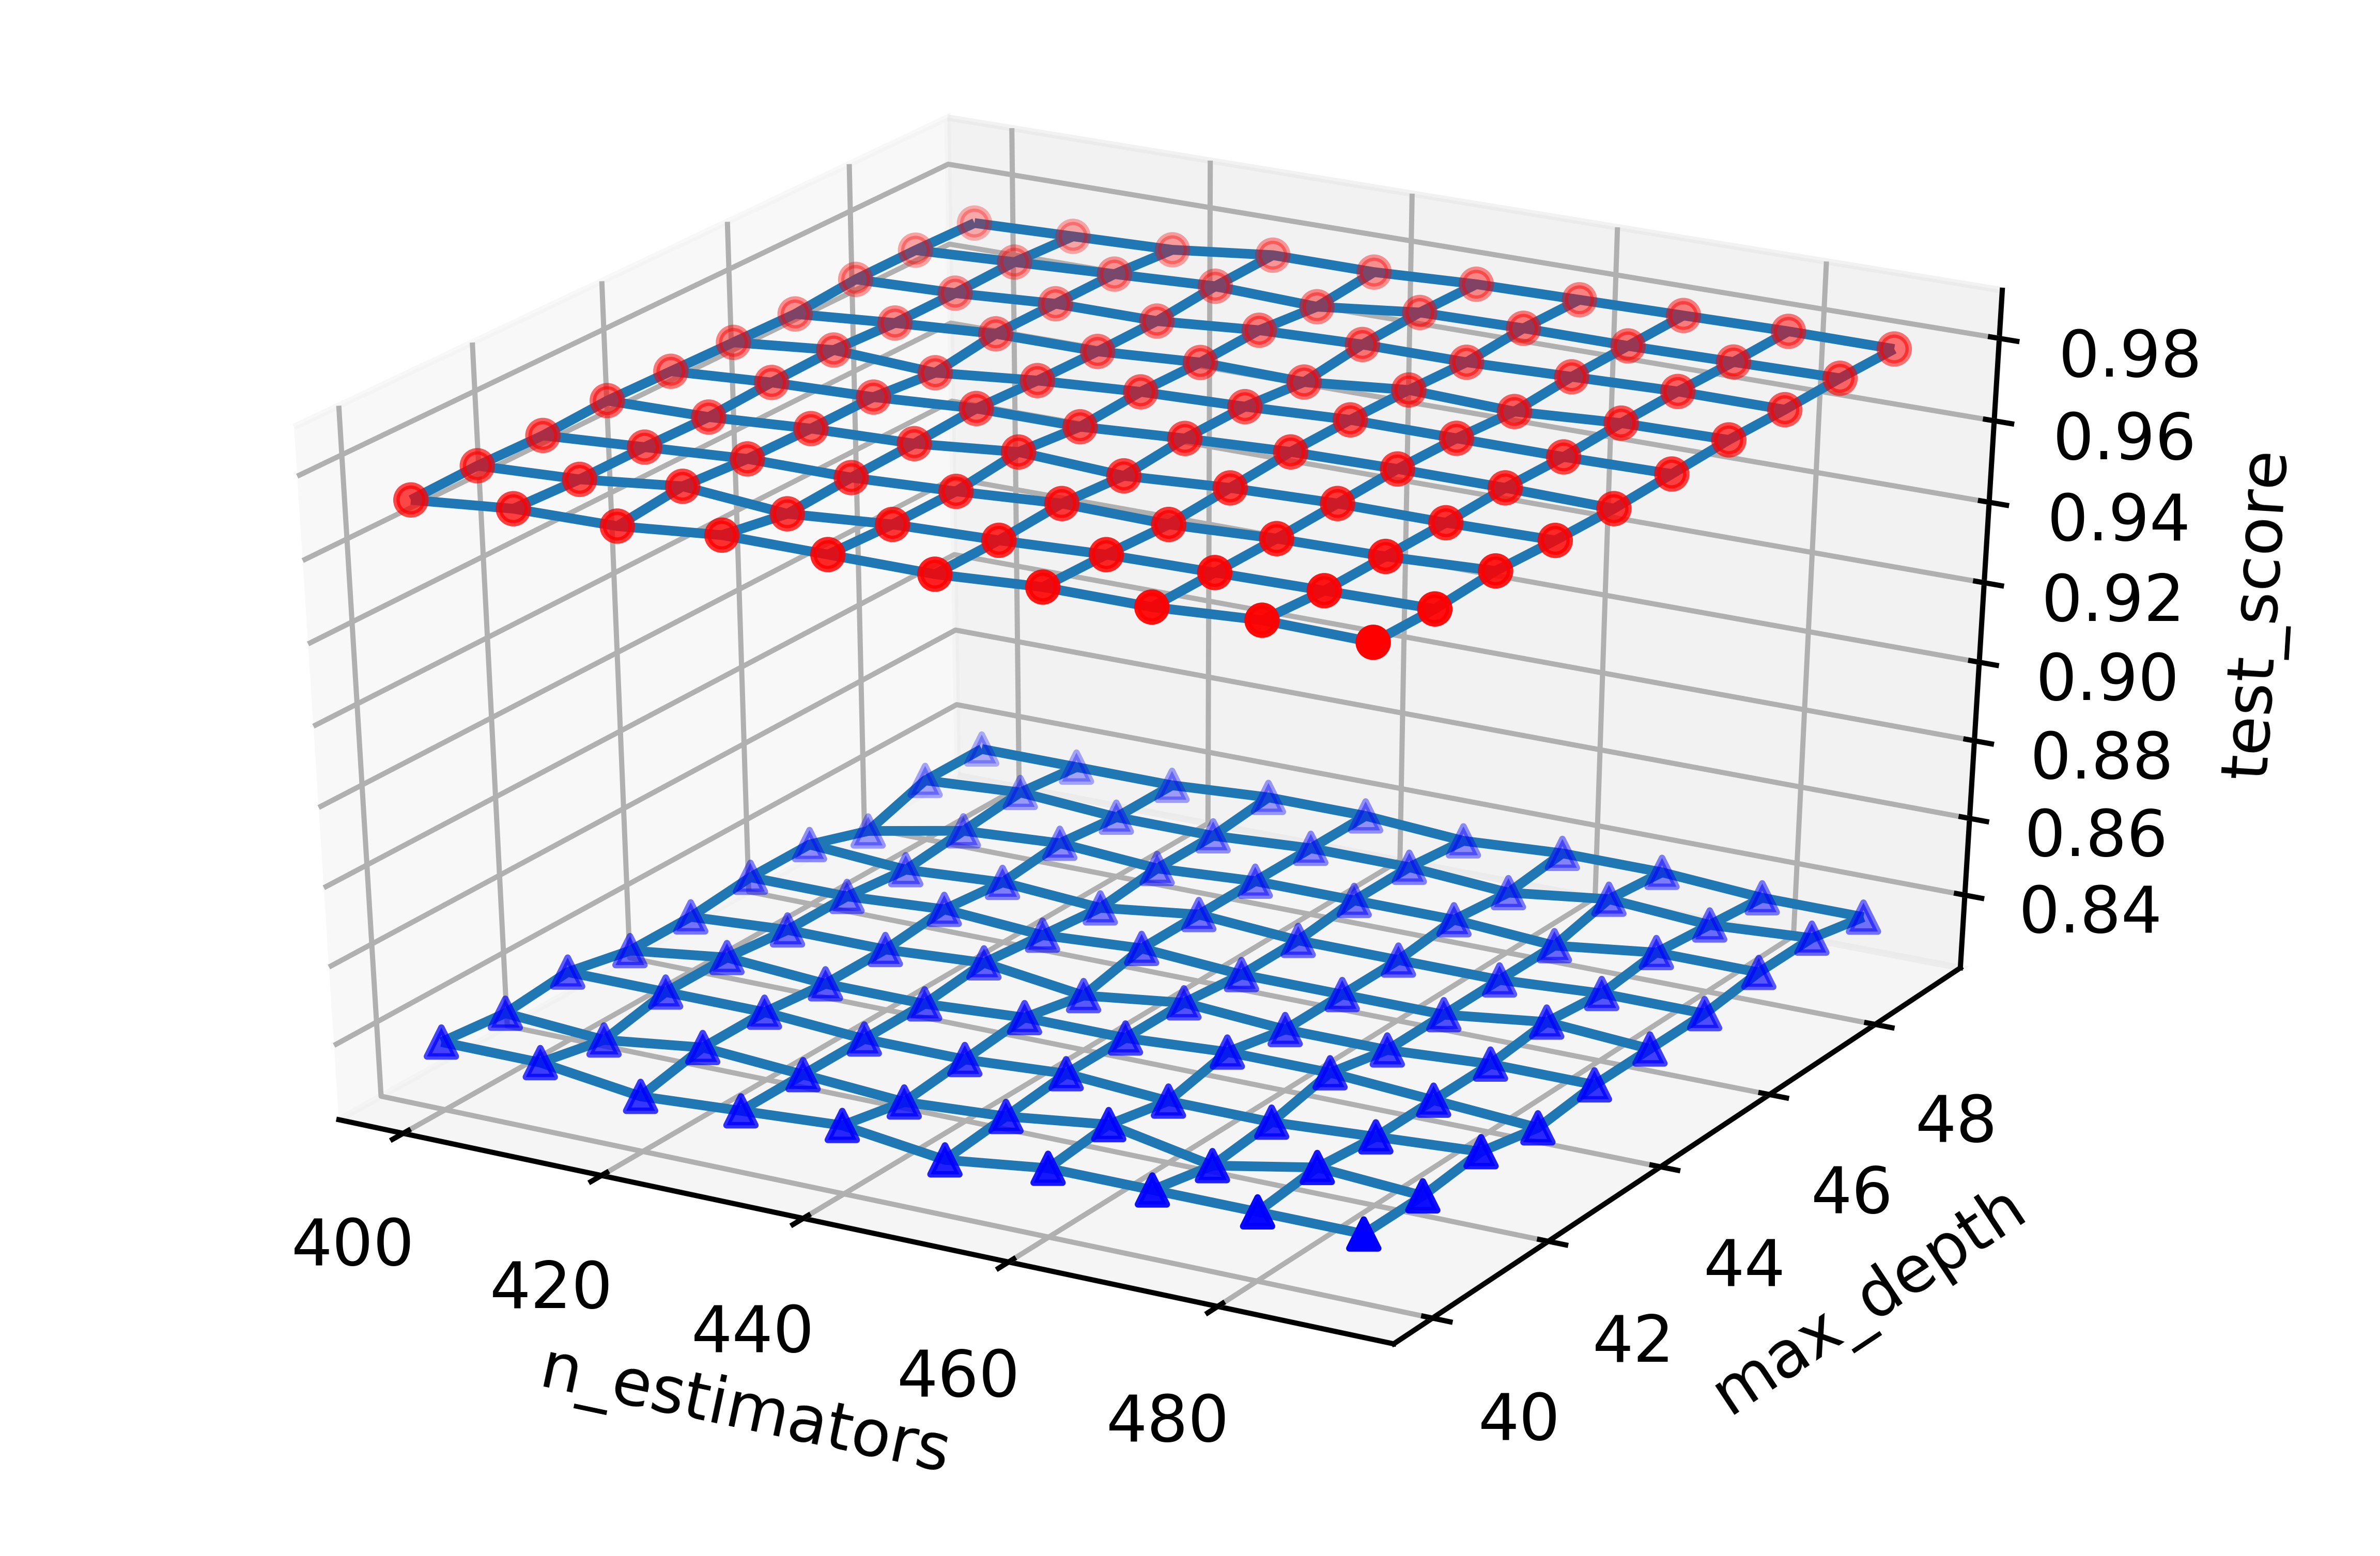
\includegraphics[width=0.48\linewidth]{hyperparameter_tuning_3}
  \caption{Max depth range from 40 to 49, and number of estimators range from 400 to 490.}
  \label{fig:results_3}
  \end{center}
\endminipage
\end{figure}

We first ran the experiment in a rough region (Figure~\ref{fig:results_1}): \verb|max_depth| range from 10 to 235 with a step of 25, while \verb|n_estimators| range from 10 to 460 with a step of 50. From this experiment we found out that when depth is larger than 60, the increasing depth of the decision tree no longer contributes to train score or test score. That is because we only have a training set of $\sim3,000$ samples, and making the tree deeper than the square root of number of samples does not contribute significantly to the accuracy of the decision trees. Then we ran 2 experiments with finer sampling (Figures~\ref{fig:results_2} and \ref{fig:results_3}). We found out from the results that we should make the depth as close to the square root of number of samples as possible, while choosing the number of estimators to be around 400, since larger numbers no longer improve the performance of the model significantly. 

\section{Discussion} 

Our general strategy focused first on feature generation, first tokenizing the data files into tags of system calls and processes ---both with and without attributes---, and then drawing features based on $n$-grams (ordered consecutive sets) of tokens, and later generalizing to $n$-bags (unordered non-consecutive sets) and $n$-tuples (ordered non-consecutive sets). Different values of $n$ (1, 2, 3, 4, and 10) were considered in the process. The features themselves were either the absolute number of occurrences of the given subsets of tokens, or their TF-IDF values to express them as a proportion of their overall occurrence. While some attributes such as certain file names proved to be of some predictive value, in the end we obtained our best results from 4-grams of system call tags.

Our model selection process considered several classifiers, including Random Forest, C-Support Vector, Linear-Support Vector and Stochastic Gradient Descent, which we tried on different subsets of the training data, and evaluating them using 5-fold cross-validation. The experimentation process showed Random Forest to be the most robust model, and we proceeded to tune its hyperparameters (number of trees in the model and their maximum depth), in order to achieve the best possible results. We also performed feature reduction by iteratively discarding features of low importance and monitoring the cross-validated scores, resulting in an optimal set of $\sim5,000$ features from an initial set of $\sim140,000$ features. One further refinement to our approach consisted in using a 2-step process in training our model, first training on 4 broad categories to predict on the 3 most frequent classes first, and then predicting separately on the 12 remaining minor classes.

Our best results on the Camelot public leaderboard were a score of 0.81632 obtained from the tuned Random Forest classifier, and then lately we improved on it by experimenting with a semi-supervised Gradient Boosting model which gave a score of 0.82263. For the final leaderboard scored on the private dataset, our best score was 0.81798, which placed us among the top 15 scores. Our placement turned out to be much better for the private dataset than for the public one, which is evidence of the robustness of our model that did not overfit the data as much as it did for other teams.

As for further improvements to our model with more time for this practical, first we would have done further experimentation with features beyond $n$-grams of system calls ---such as $n$-bags, $n$-tuples, and combinations thereof---, to result in more complex sets of features. Also, given the promise of the semi-supervised Gradient Boosting approach we discovered late in the game, we would have done further tuning of model parameters, as well as training it separately on different categories of data in a 2-step process, as we did with Random Forest.

\newpage
\nocite{rozenberg}
\bibliographystyle{apalike}
\bibliography{P2_dualspace}

\end{document}

